\label{sec:yields}
After the selections described in Section~\ref{sec:event_selection}, the event yields are extracted for signal and backgrounds for each of the four periods of \Run2, for the signal and control regions.

\subsection{Four lepton channel}
The pre-fit yields for the signal and background processes for the signal region
with four leptons passing the tight selection and a photon passing the cut-based ID (SR4P\_1P),
can be seen in Table~\ref{tab:Run2_SR4P_phoCR_lepCR} (Table~\ref{tab:Run2_SR4P_phoMC_lepCR})
when using the data-driven (simulation) to estimate the fake photon background.
The simulation of \nonprompt photons corresponds to the events without a prompt generated photon
in the samples $\PQq\PQq\to\PZ\PZ$ and $\Pg\Pg\to\PZ\PZ$.

Alternatively, the expected yields obtained using the
working point \texttt{wp90} of the MVA ID are shown in Table~\ref{tab:Run2_SR4P_phoMC_lepCR_wp90}.

Additional tables, including also the observed number of data events, are provided
for the fake photon application region (Table~\ref{tab:yields_Run2_CR4P_1F_lepCR}),
and for the fake lepton application regions (Tables~\ref{tab:yields_Run2_CR3P1F_1P} and~\ref{tab:yields_Run2_CR2P2F_1P}).

The yields in the triboson fiducial region are shown
in Table~\ref{tab:yield_SR4P_1P_FSRcut_Loose} for the Loose working point of the cut-based ID,
and in Table~\ref{tab:yield_SR4P_1P_FSRcut_wp80} when using the \texttt{wp80} of the MVA ID instead.
The yields in the subset of the fake photon application region that passes the FSR-suppressing cut,
are shown in Table~\ref{tab:yield_CR4P_1F_FSRcut}.
This region is used for the estimate of the \nonprompt photon background in the triboson fiducial region.

\begin{table}
  \caption{Yields from the signal region SR4P\_1P, with four leptons passing the tight selection and a photon passing the cut-based ID.
  The \nonprompt and misidentified photons are estimated with the data-driven method
  and thus only the events containing a prompt generated photon are included from the main background samples.
  }
  \label{tab:Run2_SR4P_phoCR_lepCR}
  % Note: this is from the variable mZZGloose
  \resizebox{\textwidth}{!}{%
  \begin{tabular}{l >{$}r<{$} >{$}r<{$} >{$}r<{$} >{$}r<{$} >{$}r<{$}}
    \toprule
    {} & \makecell[c]{\text{2016preVFP}} & \makecell[c]{\text{2016postVFP}} & \makecell[c]{\text{2017}} & \makecell[c]{\text{2018}} & \makecell[c]{\text{\Run2}}\\
    \midrule
    $\PZ\PZ\PGg\to4\Pl\PGg$       &  1.96 \pm 0.05  &  1.71 \pm 0.04  &  4.02 \pm 0.10  &   5.86 \pm 0.14  &  13.56 \pm 0.18 \\
    $\Pg\Pg\to\PZ\PZ\to4\Pe$      &  0.03 \pm 0.00  &  0.03 \pm 0.00  &  0.08 \pm 0.00  &   0.10 \pm 0.00  &   0.24 \pm 0.00 \\
    $\Pg\Pg\to\PZ\PZ\to2\Pe2\PGm$ &  0.06 \pm 0.00  &  0.06 \pm 0.00  &  0.07 \pm 0.00  &   0.10 \pm 0.00  &   0.29 \pm 0.01 \\
    $\Pg\Pg\to\PZ\PZ\to4\PGm$     &  0.06 \pm 0.00  &  0.05 \pm 0.00  &  0.12 \pm 0.00  &   0.16 \pm 0.00  &   0.38 \pm 0.01 \\
    $\PZ\PZ\PZ$                   &  0.01 \pm 0.01  &  0.00 \pm 0.00  &  0.02 \pm 0.01  &   0.03 \pm 0.01  &   0.05 \pm 0.01 \\
    $\PQt\PAQt\PZ$+jets           &  0.01 \pm 0.00  &  0.01 \pm 0.00  &  0.04 \pm 0.00  &   0.04 \pm 0.01  &   0.10 \pm 0.01 \\
    Fake photons                  &  1.36 \pm 0.65  &  1.01 \pm 0.51  &  1.37 \pm 0.52  &   2.45 \pm 0.69  &   6.19 \pm 1.20 \\
    $\PW\PZ\PZ$                   &  0.00 \pm 0.00  &  0.02 \pm 0.01  &  0.02 \pm 0.02  &   0.07 \pm 0.03  &   0.10 \pm 0.03 \\
    $\PW\PW\PZ$                   &  0.00 \pm 0.00  &  0.04 \pm 0.04  &  0.04 \pm 0.04  &   0.08 \pm 0.06  &   0.16 \pm 0.08 \\
    \noalign{\vspace{.3ex}}\hline\noalign{\vspace{.3ex}}
    Total                         &  3.49 \pm 0.66  &  2.93 \pm 0.51  &  5.76 \pm 0.53  &   8.90 \pm 0.71  &  21.07 \pm 1.22 \\
    Data                          & \makecell[c]{4} & \makecell[c]{3} & \makecell[c]{6} & \makecell[c]{11} & \makecell[c]{24}\\
    \bottomrule
  \end{tabular}
  }
\end{table}

\begin{table}
  \caption{Yields from the signal region SR4P\_1P, with four leptons passing the tight selection and a photon passing the cut-based ID.
    The \nonprompt and misidentified photons are taken from the simulation.
  }
  \label{tab:Run2_SR4P_phoMC_lepCR}
  % Note: this is from the variable mZZGloose
  \resizebox{\textwidth}{!}{%
  \begin{tabular}{l >{$}r<{$} >{$}r<{$} >{$}r<{$} >{$}r<{$} >{$}r<{$}}
    \toprule
    {} & \makecell[c]{\text{2016preVFP}} & \makecell[c]{\text{2016postVFP}} & \makecell[c]{\text{2017}} & \makecell[c]{\text{2018}} & \makecell[c]{\text{\Run2}}\\
    \midrule
    $\PZ\PZ\PGg\to4\Pl\PGg$       &  1.96 \pm 0.05  &  1.71 \pm 0.04  &  4.02 \pm 0.10  &   5.86 \pm 0.14  &  13.56 \pm 0.18 \\
    \qqZZnonpro                   &  0.24 \pm 0.01  &  0.21 \pm 0.01  &  0.61 \pm 0.02  &   0.86 \pm 0.03  &   1.92 \pm 0.03 \\
    $\Pg\Pg\to\PZ\PZ\to4\Pe$      &  0.04 \pm 0.00  &  0.03 \pm 0.00  &  0.09 \pm 0.00  &   0.12 \pm 0.00  &   0.28 \pm 0.00 \\
    $\Pg\Pg\to\PZ\PZ\to2\Pe2\PGm$ &  0.08 \pm 0.00  &  0.07 \pm 0.00  &  0.09 \pm 0.00  &   0.13 \pm 0.00  &   0.36 \pm 0.01 \\
    $\Pg\Pg\to\PZ\PZ\to4\PGm$     &  0.07 \pm 0.00  &  0.05 \pm 0.00  &  0.14 \pm 0.00  &   0.19 \pm 0.00  &   0.45 \pm 0.01 \\
    $\PZ\PZ\PZ$                   &  0.01 \pm 0.01  &  0.00 \pm 0.00  &  0.02 \pm 0.01  &   0.05 \pm 0.01  &   0.08 \pm 0.02 \\
    $\PW\PZ\PZ$                   &  0.01 \pm 0.01  &  0.03 \pm 0.01  &  0.04 \pm 0.02  &   0.09 \pm 0.03  &   0.16 \pm 0.04 \\
    $\PQt\PAQt\PZ$+jets           &  0.01 \pm 0.00  &  0.01 \pm 0.00  &  0.05 \pm 0.01  &   0.05 \pm 0.01  &   0.12 \pm 0.01 \\
    Fake leptons                  &  0.05 \pm 0.07  &  0.00 \pm 0.00  &  0.09 \pm 0.12  &   0.12 \pm 0.09  &   0.25 \pm 0.16 \\
    $\PW\PW\PZ$                   &  0.00 \pm 0.00  &  0.04 \pm 0.04  &  0.04 \pm 0.04  &   0.08 \pm 0.06  &   0.16 \pm 0.08 \\
    \noalign{\vspace{.3ex}}\hline\noalign{\vspace{.3ex}}
    Total                         &  2.46 \pm 0.08  &  2.16 \pm 0.06  &  5.18 \pm 0.16  &   7.56 \pm 0.18  &  17.36 \pm 0.27 \\
    Data                          & \makecell[c]{4} & \makecell[c]{3} & \makecell[c]{6} & \makecell[c]{11} & \makecell[c]{24}\\
    \bottomrule
  \end{tabular}
  }
\end{table}

\begin{table}
  \caption{Yields from the signal region SR4P\_1P, with four leptons passing the tight selection
  and a photon passing the \texttt{wp90} of the MVA based ID.
  The \nonprompt and misidentified photons are taken from the simulation.
  }
  \label{tab:Run2_SR4P_phoMC_lepCR_wp90}
  % Note: this is from the variable mZZGloose
  \resizebox{\textwidth}{!}{%
  \begin{tabular}{l >{$}r<{$} >{$}r<{$} >{$}r<{$} >{$}r<{$} >{$}r<{$}}
    \toprule
    {} & \makecell[c]{\text{2016preVFP}} & \makecell[c]{\text{2016postVFP}} & \makecell[c]{\text{2017}} & \makecell[c]{\text{2018}} & \makecell[c]{\text{\Run2}}\\
    \midrule
    $\PZ\PZ\PGg\to4\Pl\PGg$       &  2.03 \pm 0.05  &  1.78 \pm 0.04  &  4.29 \pm 0.10  &   6.13 \pm 0.14  &  14.23 \pm 0.19 \\
    \qqZZnonpro                   &  0.19 \pm 0.01  &  0.16 \pm 0.01  &  0.45 \pm 0.02  &   0.65 \pm 0.02  &   1.45 \pm 0.03 \\
    $\Pg\Pg\to\PZ\PZ\to4\Pe$      &  0.04 \pm 0.00  &  0.03 \pm 0.00  &  0.09 \pm 0.00  &   0.12 \pm 0.00  &   0.28 \pm 0.00 \\
    $\Pg\Pg\to\PZ\PZ\to2\Pe2\PGm$ &  0.08 \pm 0.00  &  0.07 \pm 0.00  &  0.09 \pm 0.00  &   0.13 \pm 0.00  &   0.36 \pm 0.01 \\
    $\Pg\Pg\to\PZ\PZ\to4\PGm$     &  0.07 \pm 0.00  &  0.05 \pm 0.00  &  0.14 \pm 0.00  &   0.19 \pm 0.00  &   0.45 \pm 0.01 \\
    $\PZ\PZ\PZ$                   &  0.01 \pm 0.01  &  0.00 \pm 0.00  &  0.02 \pm 0.01  &   0.04 \pm 0.01  &   0.08 \pm 0.02 \\
    $\PQt\PAQt\PZ$+jets           &  0.01 \pm 0.00  &  0.01 \pm 0.00  &  0.05 \pm 0.01  &   0.06 \pm 0.01  &   0.13 \pm 0.01 \\
    Fake leptons                  &  0.04 \pm 0.07  &  0.10 \pm 0.12  &  0.11 \pm 0.12  &   0.02 \pm 0.08  &   0.28 \pm 0.20 \\
    $\PW\PZ\PZ$                   &  0.00 \pm 0.00  &  0.02 \pm 0.01  &  0.06 \pm 0.02  &   0.08 \pm 0.03  &   0.16 \pm 0.04 \\
    $\PW\PW\PZ$                   &  0.00 \pm 0.00  &  0.00 \pm 0.00  &  0.04 \pm 0.04  &   0.08 \pm 0.06  &   0.12 \pm 0.07 \\
    \noalign{\vspace{.3ex}}\hline\noalign{\vspace{.3ex}}
    Total                         &  2.46 \pm 0.08  &  2.23 \pm 0.12  &  5.34 \pm 0.16  &   7.49 \pm 0.18  &  17.53 \pm 0.28 \\
    Data                          & \makecell[c]{3} & \makecell[c]{3} & \makecell[c]{6} & \makecell[c]{11} & \makecell[c]{23}\\
    \bottomrule
  \end{tabular}
  }
\end{table}

\begin{table}
\caption{Yields from the fake photon application region CR4P\_1F, with four leptons passing the tight selection and a photon passing the VeryLoose ID but failing the cut-based ID Loose.}
\label{tab:yields_Run2_CR4P_1F_lepCR}
\resizebox{\textwidth}{!}{%
  \begin{tabular}{l >{$}r<{$} >{$}r<{$} >{$}r<{$} >{$}r<{$} >{$}r<{$}}
    \toprule
    {} & \makecell[c]{\text{2016preVFP}} & \makecell[c]{\text{2016postVFP}} & \makecell[c]{\text{2017}} & \makecell[c]{\text{2018}} & \makecell[c]{\text{\Run2}}\\
    \midrule
    $\PZ\PZ\PGg\to4\Pl\PGg$       &  0.30 \pm 0.02  &  0.29 \pm 0.02  &  0.84 \pm 0.05  &   1.19 \pm 0.06  &   2.62 \pm 0.08 \\
    \qqZZnonpro                   &  2.40 \pm 0.03  &  2.28 \pm 0.03  &  6.43 \pm 0.06  &   9.51 \pm 0.08  &  20.62 \pm 0.11 \\
    $\Pg\Pg\to\PZ\PZ\to4\Pe$      &  0.06 \pm 0.00  &  0.06 \pm 0.00  &  0.17 \pm 0.00  &   0.26 \pm 0.00  &   0.55 \pm 0.01 \\
    $\Pg\Pg\to\PZ\PZ\to2\Pe2\PGm$ &  0.16 \pm 0.00  &  0.16 \pm 0.00  &  0.22 \pm 0.01  &   0.32 \pm 0.01  &   0.86 \pm 0.01 \\
    $\Pg\Pg\to\PZ\PZ\to4\PGm$     &  0.11 \pm 0.00  &  0.09 \pm 0.00  &  0.25 \pm 0.00  &   0.38 \pm 0.01  &   0.84 \pm 0.01 \\
    $\PZ\PZ\PZ$                   &  0.04 \pm 0.01  &  0.02 \pm 0.01  &  0.07 \pm 0.02  &   0.07 \pm 0.02  &   0.20 \pm 0.03 \\
    $\PW\PZ\PZ$                   &  0.06 \pm 0.02  &  0.07 \pm 0.02  &  0.12 \pm 0.03  &   0.12 \pm 0.04  &   0.38 \pm 0.06 \\
    $\PW\PW\PZ$                   &  0.05 \pm 0.05  &  0.05 \pm 0.05  &  0.00 \pm 0.00  &   0.04 \pm 0.04  &   0.13 \pm 0.08 \\
    $\PQt\PAQt\PZ$+jets           &  0.06 \pm 0.01  &  0.05 \pm 0.00  &  0.17 \pm 0.01  &   0.25 \pm 0.02  &   0.53 \pm 0.02 \\
    Fake leptons                  &  0.03 \pm 0.05  &  0.05 \pm 0.05  &  0.06 \pm 0.09  &   0.05 \pm 0.10  &   0.19 \pm 0.15 \\
    \noalign{\vspace{.3ex}}\hline\noalign{\vspace{.3ex}}
    Total                         &  3.26 \pm 0.08  &  3.13 \pm 0.08  &  8.33 \pm 0.12  &  12.19 \pm 0.15  &  26.91 \pm 0.23 \\
    Data                          & \makecell[c]{5} & \makecell[c]{4} & \makecell[c]{7} & \makecell[c]{13} & \makecell[c]{29}\\
    \bottomrule
  \end{tabular}
  }
\end{table}

\begin{table}
\caption{Yields in CR3P1F\_1P, one of the fake lepton application regions, with three leptons passing the tight selection, one passing only a loose selection, and a photon passing the cut-based ID.}
\label{tab:yields_Run2_CR3P1F_1P}
\resizebox{\textwidth}{!}{%
  \begin{tabular}{l >{$}r<{$} >{$}r<{$} >{$}r<{$} >{$}r<{$} >{$}r<{$}}
    \toprule
    {} & \makecell[c]{\text{2016preVFP}} & \makecell[c]{\text{2016postVFP}} & \makecell[c]{\text{2017}} & \makecell[c]{\text{2018}} & \makecell[c]{\text{\Run2}}\\
    \midrule
    $\PZ\PZ\PGg\to4\Pl\PGg$       &  0.14 \pm 0.01  &  0.14 \pm 0.01  &  0.39 \pm 0.03  &  0.51 \pm 0.04  &  1.18 \pm 0.05 \\
    $\PW\PZ\PGg\to3\Pl\PGn\PGg$   &  0.21 \pm 0.01  &  0.19 \pm 0.01  &  0.42 \pm 0.02  &  0.71 \pm 0.03  &  1.53 \pm 0.04 \\
    $\PZ\PGg\to\Pl\Pl$            &  0.75 \pm 0.28  &  0.00 \pm 0.00  &  0.46 \pm 0.39  &  0.49 \pm 0.45  &  1.70 \pm 0.66 \\
    \qqZZnonpro                   &  0.10 \pm 0.01  &  0.09 \pm 0.01  &  0.23 \pm 0.01  &  0.33 \pm 0.02  &  0.75 \pm 0.02 \\
    $\Pg\Pg\to\PZ\PZ\to4\Pe$      &  0.01 \pm 0.00  &  0.01 \pm 0.00  &  0.02 \pm 0.00  &  0.04 \pm 0.00  &  0.08 \pm 0.00 \\
    $\Pg\Pg\to\PZ\PZ\to2\Pe2\PGm$ &  0.01 \pm 0.00  &  0.01 \pm 0.00  &  0.02 \pm 0.00  &  0.02 \pm 0.00  &  0.06 \pm 0.00 \\
    $\Pg\Pg\to\PZ\PZ\to4\PGm$     &  0.00 \pm 0.00  &  0.00 \pm 0.00  &  0.01 \pm 0.00  &  0.01 \pm 0.00  &  0.02 \pm 0.00 \\
    \WZnonpro                     &  0.05 \pm 0.03  &  0.03 \pm 0.03  &  0.13 \pm 0.09  &  1.10 \pm 0.32  &  1.32 \pm 0.33 \\
    $\PZ\PZ\PZ$                   &  0.00 \pm 0.00  &  0.00 \pm 0.00  &  0.01 \pm 0.01  &  0.01 \pm 0.01  &  0.02 \pm 0.01 \\
    $\PW\PZ\PZ$                   &  0.01 \pm 0.01  &  0.00 \pm 0.00  &  0.00 \pm 0.01  &  0.01 \pm 0.01  &  0.02 \pm 0.02 \\
    $\PQt\PAQt\PZ$+jets           &  0.04 \pm 0.00  &  0.04 \pm 0.00  &  0.07 \pm 0.01  &  0.11 \pm 0.01  &  0.26 \pm 0.01 \\
    \DYnonpro                     &  0.00 \pm 0.00  &  0.00 \pm 0.00  &  0.00 \pm 0.00  &  0.68 \pm 3.52  &  0.68 \pm 3.52 \\
    \noalign{\vspace{.3ex}}\hline\noalign{\vspace{.3ex}}
    Total                         &  1.34 \pm 0.29  &  0.51 \pm 0.03  &  1.76 \pm 0.40  &  4.02 \pm 3.56  &  7.63 \pm 3.60 \\
    Data                          & \makecell[c]{1} & \makecell[c]{0} & \makecell[c]{2} & \makecell[c]{5} & \makecell[c]{8}\\
    \bottomrule
  \end{tabular}
  }
\end{table}

\begin{table}
\caption{Yields in CR2P2F\_1P, one of the fake lepton application regions, with two leptons passing the tight selection, two passing only a loose selection, and a photon passing the cut-based ID.}
\label{tab:yields_Run2_CR2P2F_1P}
\resizebox{\textwidth}{!}{%
  \begin{tabular}{l >{$}r<{$} >{$}r<{$} >{$}r<{$} >{$}r<{$} >{$}r<{$}}
    \toprule
    {} & \makecell[c]{\text{2016preVFP}} & \makecell[c]{\text{2016postVFP}} & \makecell[c]{\text{2017}} & \makecell[c]{\text{2018}} & \makecell[c]{\text{\Run2}}\\
    \midrule
    $\PZ\PZ\PGg\to4\Pl\PGg$       &  0.01 \pm 0.00  &  0.00 \pm 0.00  &   0.01 \pm 0.00  &    0.03 \pm 0.01 &    0.05 \pm 0.01 \\
    $\PW\PZ\PGg\to3\Pl\PGn\PGg$   &  0.02 \pm 0.00  &  0.02 \pm 0.00  &   0.03 \pm 0.01  &    0.05 \pm 0.01 &    0.13 \pm 0.01 \\
    \DYnonpro                     &  6.23 \pm 3.60  &  1.85 \pm 1.85  &  15.81 \pm 5.60  &  37.76 \pm 15.47 &  61.66 \pm 16.94 \\
    $\PZ\PGg\to\Pl\Pl$            &  6.60 \pm 0.80  &  0.00 \pm 0.00  &  13.78 \pm 1.46  &   22.22 \pm 2.34 &   42.61 \pm 2.87 \\
    \qqZZnonpro                   &  0.01 \pm 0.00  &  0.01 \pm 0.00  &   0.01 \pm 0.00  &    0.02 \pm 0.00 &    0.05 \pm 0.01 \\
    $\Pg\Pg\to\PZ\PZ\to4\Pe$      &  0.00 \pm 0.00  &  0.00 \pm 0.00  &   0.00 \pm 0.00  &    0.00 \pm 0.00 &    0.00 \pm 0.00 \\
    $\Pg\Pg\to\PZ\PZ\to2\Pe2\PGm$ &  0.00 \pm 0.00  &  0.00 \pm 0.00  &   0.00 \pm 0.00  &    0.00 \pm 0.00 &    0.00 \pm 0.00 \\
    \WZnonpro                     &  0.00 \pm 0.02  &  0.03 \pm 0.02  &   0.12 \pm 0.08  &    0.15 \pm 0.14 &    0.30 \pm 0.16 \\
    $\PQt\PAQt\PZ$+jets           &  0.02 \pm 0.00  &  0.02 \pm 0.00  &   0.03 \pm 0.00  &    0.05 \pm 0.01 &    0.13 \pm 0.01 \\
    $\PQt\PZ\PQq$                 &  0.00 \pm 0.01  &  0.00 \pm 0.01  &   0.02 \pm 0.01  &    0.02 \pm 0.01 &    0.05 \pm 0.02 \\
    $\PQt\PW$                     &  0.06 \pm 0.06  &  0.00 \pm 0.00  &   0.09 \pm 0.10  &    0.00 \pm 0.00 &    0.14 \pm 0.11 \\
    $\Pg\Pg\to\PZ\PZ\to4\PGm$     &  0.00 \pm 0.00  &  0.00 \pm 0.00  &   0.00 \pm 0.00  &    0.00 \pm 0.00 &    0.00 \pm 0.00 \\
    \noalign{\vspace{.3ex}}\hline\noalign{\vspace{.3ex}}
    Total                         & 12.96 \pm 3.69  &  1.94 \pm 1.85  &  29.91 \pm 5.79  &  60.33 \pm 15.65 & 105.13 \pm 17.19 \\
    Data                          & \makecell[c]{17}& \makecell[c]{9} & \makecell[c]{23} & \makecell[c]{28} & \makecell[c]{77} \\
    \bottomrule
  \end{tabular}
  }
\end{table}

\begin{table}
  \caption{Yields in the fiducial triboson region of the four lepton channel, using the cut-based ID selection for the photon.
  \Nonprompt and misidentified photons are estimated from data.}
  \label{tab:yield_SR4P_1P_FSRcut_Loose_phoCR}
  \resizebox{\textwidth}{!}{%
  \begin{tabular}{l >{$}r<{$} >{$}r<{$} >{$}r<{$} >{$}r<{$} >{$}r<{$}}
    \toprule
    {} & \makecell[c]{\text{2016preVFP}} & \makecell[c]{\text{2016postVFP}} & \makecell[c]{\text{2017}} & \makecell[c]{\text{2018}} & \makecell[c]{\text{\Run2}}\\
    \midrule
    $\PZ\PZ\PGg\to4\Pl\PGg$       &  0.84 \pm 0.03  &  0.73 \pm 0.03  &  1.76 \pm 0.07  &  2.48 \pm 0.09  &  5.81 \pm 0.12 \\
    $\Pg\Pg\to\PZ\PZ\to4\PGm$     &  0.01 \pm 0.00  &  0.01 \pm 0.00  &  0.01 \pm 0.00  &  0.02 \pm 0.00  &  0.05 \pm 0.00 \\
    $\Pg\Pg\to\PZ\PZ\to2\Pe2\PGm$ &  0.01 \pm 0.00  &  0.01 \pm 0.00  &  0.01 \pm 0.00  &  0.01 \pm 0.00  &  0.04 \pm 0.00 \\
    $\Pg\Pg\to\PZ\PZ\to4\Pe$      &  0.01 \pm 0.00  &  0.01 \pm 0.00  &  0.02 \pm 0.00  &  0.03 \pm 0.00  &  0.08 \pm 0.00 \\
    $\PZ\PZ\PZ$                   &  0.00 \pm 0.00  &  0.00 \pm 0.00  &  0.01 \pm 0.01  &  0.01 \pm 0.01  &  0.03 \pm 0.01 \\
    $\PQt\PAQt\PZ$+jets           &  0.01 \pm 0.00  &  0.00 \pm 0.00  &  0.02 \pm 0.00  &  0.02 \pm 0.00  &  0.04 \pm 0.01 \\
    Fake photons                  &  1.06 \pm 0.59  &  0.00 \pm 0.00  &  0.00 \pm 0.00  &  2.24 \pm 0.66  &  3.30 \pm 0.88 \\
    $\PW\PZ\PZ$                   &  0.00 \pm 0.00  &  0.01 \pm 0.01  &  0.00 \pm 0.01  &  0.05 \pm 0.02  &  0.05 \pm 0.03 \\
    \noalign{\vspace{.3ex}}\hline\noalign{\vspace{.3ex}}
    Total                         &  1.94 \pm 0.59  &  0.76 \pm 0.03  &  1.84 \pm 0.07  &  4.87 \pm 0.67  &  9.41 \pm 0.89 \\
    Data                          & \makecell[c]{1} & \makecell[c]{0} & \makecell[c]{0} & \makecell[c]{6} & \makecell[c]{7}\\
    \bottomrule
  \end{tabular}
  }
\end{table}

\begin{table}
  \caption{Yields in the fiducial triboson region of the four lepton channel, using the cut-based ID selection for the photon.
  The fake photon background is estimated from simulation.}
  \label{tab:yield_SR4P_1P_FSRcut_Loose}
  \resizebox{\textwidth}{!}{%
  \begin{tabular}{l >{$}r<{$} >{$}r<{$} >{$}r<{$} >{$}r<{$} >{$}r<{$}}
    \toprule
    {} & \makecell[c]{\text{2016preVFP}} & \makecell[c]{\text{2016postVFP}} & \makecell[c]{\text{2017}} & \makecell[c]{\text{2018}} & \makecell[c]{\text{\Run2}}\\
    \midrule
    $\PZ\PZ\PGg\to4\Pl\PGg$       &  0.84 \pm 0.03  &  0.73 \pm 0.03  &  1.76 \pm 0.07  &  2.48 \pm 0.09  &  5.81 \pm 0.12 \\
    \qqZZnonpro                   &  0.20 \pm 0.01  &  0.17 \pm 0.01  &  0.50 \pm 0.02  &  0.70 \pm 0.02  &  1.57 \pm 0.03 \\
    Fake leptons                  &  0.06 \pm 0.07  &  0.00 \pm 0.00  &  0.11 \pm 0.11  &  0.10 \pm 0.09  &  0.27 \pm 0.16 \\
    $\Pg\Pg\to\PZ\PZ\to4\Pe$      &  0.01 \pm 0.00  &  0.01 \pm 0.00  &  0.02 \pm 0.00  &  0.04 \pm 0.00  &  0.08 \pm 0.00 \\
    $\Pg\Pg\to\PZ\PZ\to2\Pe2\PGm$ &  0.02 \pm 0.00  &  0.02 \pm 0.00  &  0.02 \pm 0.00  &  0.03 \pm 0.00  &  0.09 \pm 0.00 \\
    $\Pg\Pg\to\PZ\PZ\to4\PGm$     &  0.02 \pm 0.00  &  0.02 \pm 0.00  &  0.04 \pm 0.00  &  0.06 \pm 0.00  &  0.14 \pm 0.00 \\
    $\PZ\PZ\PZ$                   &  0.00 \pm 0.00  &  0.00 \pm 0.00  &  0.01 \pm 0.01  &  0.03 \pm 0.01  &  0.05 \pm 0.01 \\
    $\PW\PZ\PZ$                   &  0.00 \pm 0.00  &  0.01 \pm 0.01  &  0.02 \pm 0.02  &  0.07 \pm 0.03  &  0.11 \pm 0.03 \\
    $\PQt\PAQt\PZ$+jets           &  0.01 \pm 0.00  &  0.00 \pm 0.00  &  0.02 \pm 0.00  &  0.02 \pm 0.00  &  0.05 \pm 0.01 \\
    \noalign{\vspace{.3ex}}\hline\noalign{\vspace{.3ex}}
    Total                         &  1.16 \pm 0.07  &  0.96 \pm 0.03  &  2.52 \pm 0.13  &  3.54 \pm 0.13  &  8.18 \pm 0.20 \\
    Data                          & \makecell[c]{1} & \makecell[c]{0} & \makecell[c]{0} & \makecell[c]{6} & \makecell[c]{7}\\
    \bottomrule
  \end{tabular}
  }
\end{table}

\begin{table}
  \caption{Yields in the fiducial triboson region of the four lepton channel, using the \texttt{wp80} of the MVA ID selection for the photon.}
  \label{tab:yield_SR4P_1P_FSRcut_wp80}
  \resizebox{\textwidth}{!}{%
  \begin{tabular}{l >{$}r<{$} >{$}r<{$} >{$}r<{$} >{$}r<{$} >{$}r<{$}}
    \toprule
    {} &  \makecell[c]{\text{2016preVFP}} & \makecell[c]{\text{2016postVFP}} & \makecell[c]{\text{2017}} & \makecell[c]{\text{2018}} & \makecell[c]{\text{\Run2}}\\
    \midrule
    $\PZ\PZ\PGg\to4\Pl\PGg$       &  0.80 \pm 0.03  &  0.69 \pm 0.03  &  1.70 \pm 0.06  &  2.37 \pm 0.09  &  5.58 \pm 0.12 \\
    \qqZZnonpro                   &  0.09 \pm 0.01  &  0.07 \pm 0.00  &  0.21 \pm 0.01  &  0.29 \pm 0.01  &  0.66 \pm 0.02 \\
    $\Pg\Pg\to\PZ\PZ\to4\Pe$      &  0.01 \pm 0.00  &  0.01 \pm 0.00  &  0.02 \pm 0.00  &  0.03 \pm 0.00  &  0.06 \pm 0.00 \\
    $\Pg\Pg\to\PZ\PZ\to2\Pe2\PGm$ &  0.01 \pm 0.00  &  0.01 \pm 0.00  &  0.02 \pm 0.00  &  0.02 \pm 0.00  &  0.06 \pm 0.00 \\
    $\Pg\Pg\to\PZ\PZ\to4\PGm$     &  0.01 \pm 0.00  &  0.01 \pm 0.00  &  0.03 \pm 0.00  &  0.04 \pm 0.00  &  0.10 \pm 0.00 \\
    $\PZ\PZ\PZ$                   &  0.00 \pm 0.00  &  0.00 \pm 0.00  &  0.01 \pm 0.01  &  0.02 \pm 0.01  &  0.04 \pm 0.01 \\
    $\PQt\PAQt\PZ$+jets           &  0.01 \pm 0.00  &  0.01 \pm 0.00  &  0.02 \pm 0.00  &  0.02 \pm 0.00  &  0.05 \pm 0.01 \\
    Fake leptons                  &  0.06 \pm 0.07  &  0.00 \pm 0.00  &  0.11 \pm 0.11  &  0.05 \pm 0.08  &  0.23 \pm 0.15 \\
    $\PW\PZ\PZ$                   &  0.00 \pm 0.00  &  0.01 \pm 0.01  &  0.04 \pm 0.02  &  0.04 \pm 0.02  &  0.09 \pm 0.03 \\
    \noalign{\vspace{.3ex}}\hline\noalign{\vspace{.3ex}}
    Total                         &  1.00 \pm 0.07  &  0.81 \pm 0.03  &  2.15 \pm 0.13  &  2.90 \pm 0.12  &  6.85 \pm 0.20 \\
    Data                          & \makecell[c]{1} & \makecell[c]{0} & \makecell[c]{1} & \makecell[c]{5} & \makecell[c]{7}\\
    \bottomrule
  \end{tabular}
  }
\end{table}

\begin{table}
  \caption{Yields in the subset of the fake photon application region in the four lepton channel,
    after the application of cut designed to suppress the FSR.
  }
  \label{tab:yield_CR4P_1F_FSRcut}
  \resizebox{\textwidth}{!}{%
  \begin{tabular}{l >{$}r<{$} >{$}r<{$} >{$}r<{$} >{$}r<{$} >{$}r<{$}}
    {} &  \makecell[c]{\text{2016preVFP}} & \makecell[c]{\text{2016postVFP}} & \makecell[c]{\text{2017}} & \makecell[c]{\text{2018}} & \makecell[c]{\text{\Run2}}\\
    \toprule
    $\PZ\PZ\PGg\to4\Pl\PGg$       &  0.17 \pm 0.01 &  0.15 \pm 0.01 &  0.45 \pm 0.03 &   0.65 \pm 0.05 &   1.42 \pm 0.06 \\
    \qqZZnonpro                   &  2.12 \pm 0.03 &  2.03 \pm 0.03 &  5.72 \pm 0.05 &   8.44 \pm 0.08 &  18.31 \pm 0.10 \\
    $\Pg\Pg\to\PZ\PZ\to4\Pe$      &  0.05 \pm 0.00 &  0.04 \pm 0.00 &  0.13 \pm 0.00 &   0.19 \pm 0.00 &   0.41 \pm 0.01 \\
    $\Pg\Pg\to\PZ\PZ\to2\Pe2\PGm$ &  0.13 \pm 0.00 &  0.14 \pm 0.00 &  0.19 \pm 0.00 &   0.28 \pm 0.01 &   0.74 \pm 0.01 \\
    $\Pg\Pg\to\PZ\PZ\to4\PGm$     &  0.08 \pm 0.00 &  0.07 \pm 0.00 &  0.19 \pm 0.00 &   0.31 \pm 0.01 &   0.66 \pm 0.01 \\
    $\PZ\PZ\PZ$                   &  0.03 \pm 0.01 &  0.02 \pm 0.01 &  0.07 \pm 0.02 &   0.06 \pm 0.02 &   0.18 \pm 0.03 \\
    $\PW\PZ\PZ$                   &  0.06 \pm 0.02 &  0.06 \pm 0.02 &  0.08 \pm 0.03 &   0.08 \pm 0.03 &   0.28 \pm 0.05 \\
    $\PQt\PAQt\PZ$+jets           &  0.03 \pm 0.00 &  0.03 \pm 0.00 &  0.09 \pm 0.01 &   0.13 \pm 0.01 &   0.28 \pm 0.01 \\
    Fake leptons                  &  0.01 \pm 0.04 &  0.00 \pm 0.00 &  0.08 \pm 0.08 &   0.03 \pm 0.05 &   0.13 \pm 0.10 \\
    $\PW\PW\PZ$                   &  0.00 \pm 0.00 &  0.05 \pm 0.05 &  0.00 \pm 0.00 &   0.00 \pm 0.00 &   0.05 \pm 0.05 \\
    \noalign{\vspace{.3ex}}\hline\noalign{\vspace{.3ex}}
    Total                         &  2.68 \pm 0.06 &  2.60 \pm 0.06 &  7.01 \pm 0.11 &  10.17 \pm 0.11 &  22.45 \pm 0.18 \\
    Data                          &\makecell[c]{4} &\makecell[c]{3} &\makecell[c]{6} &\makecell[c]{12} &\makecell[c]{25} \\
    \bottomrule
  \end{tabular}
  }
\end{table}

%% Several kinematic distributions are also studied using selections that are orthogonal to the signal region.

%% The kinematics of the photons associated with a charged lepton
%% as part of the FSR recovery algorithm (see Section~\ref{sec:FSRphotons})
%% are shown in Figure~\ref{fig:Run2_SR4P_fsrPhotons}.

%% \begin{figure}
%% \subfigure [2016preVFP ] {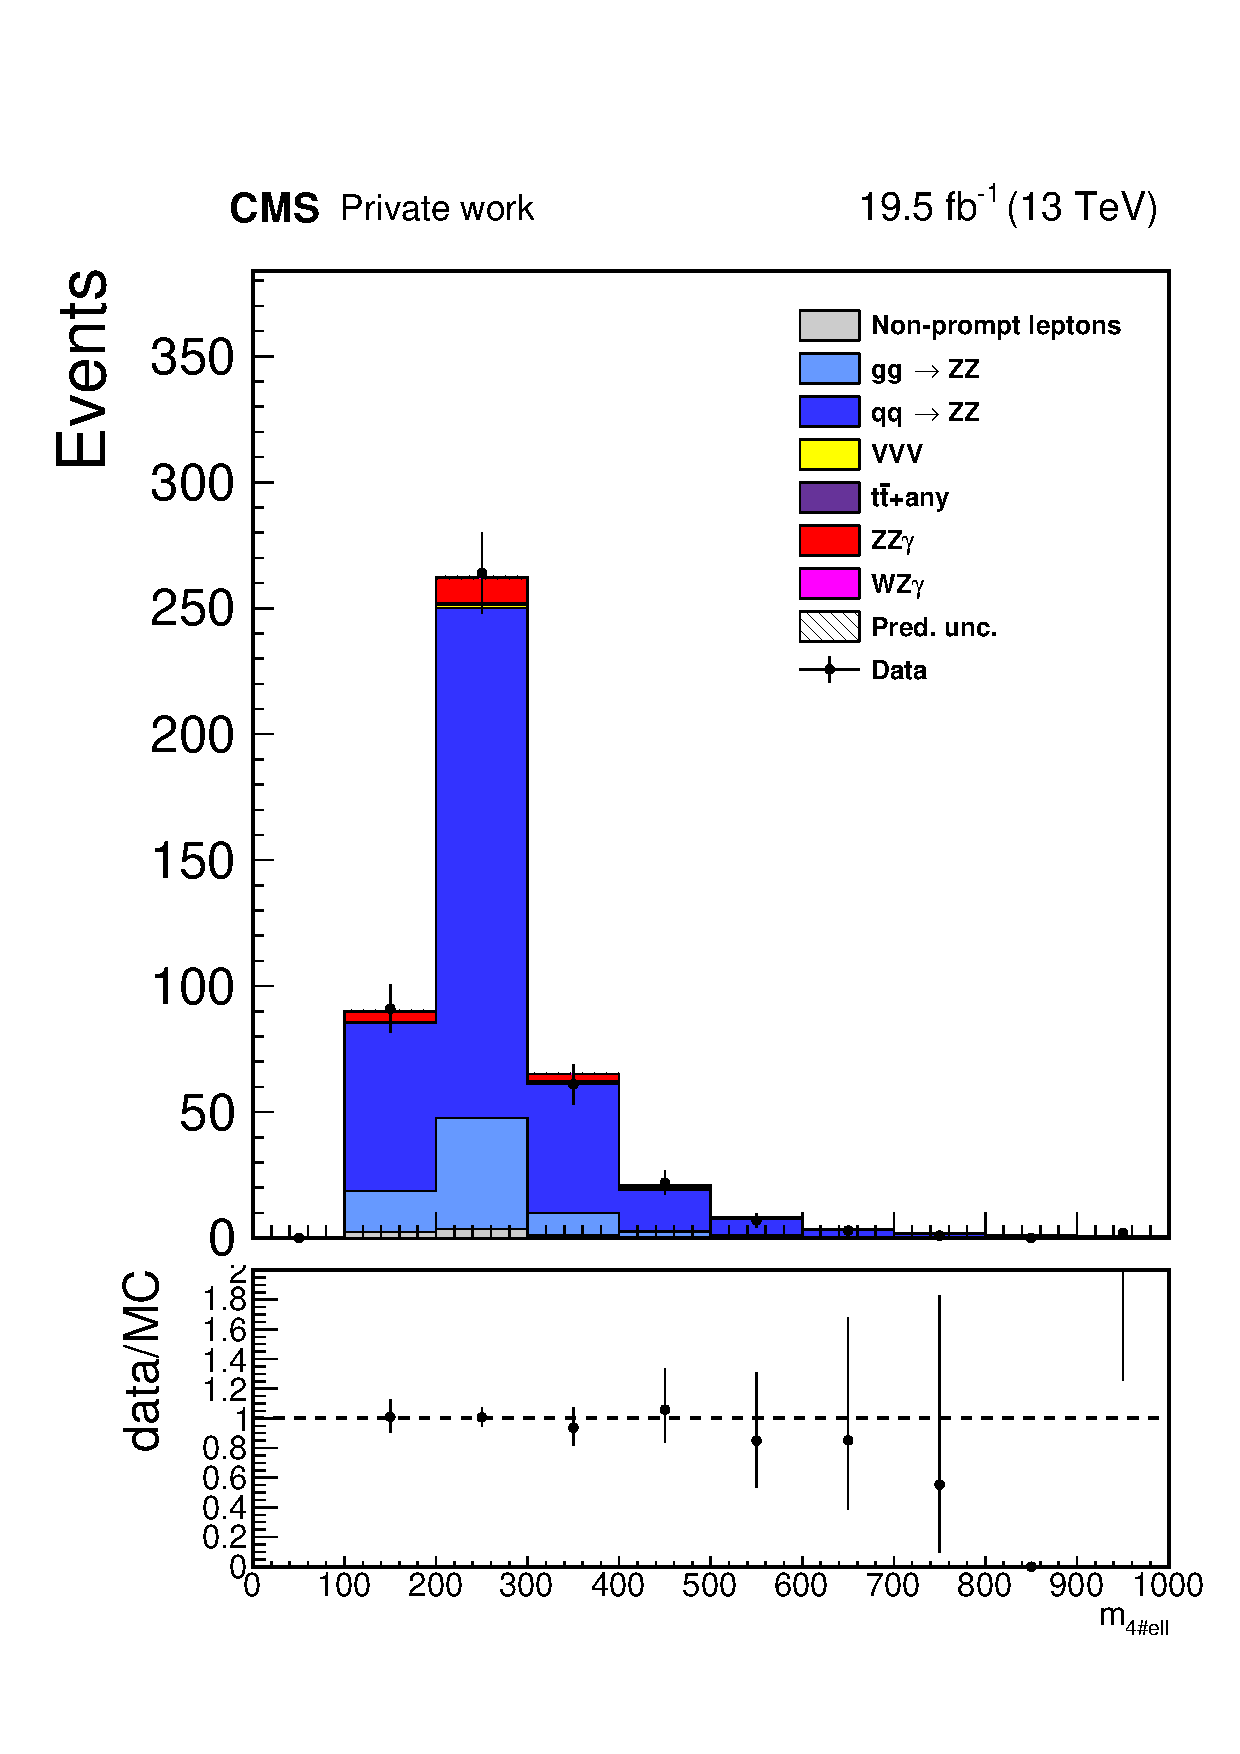
\includegraphics[width=.25\textwidth]{Figures/VVGammaAnalyzer/2016preVFP/lepCR/SR4P/ZZ_mass_pow.pdf}}%
%% \subfigure [2016postVFP] {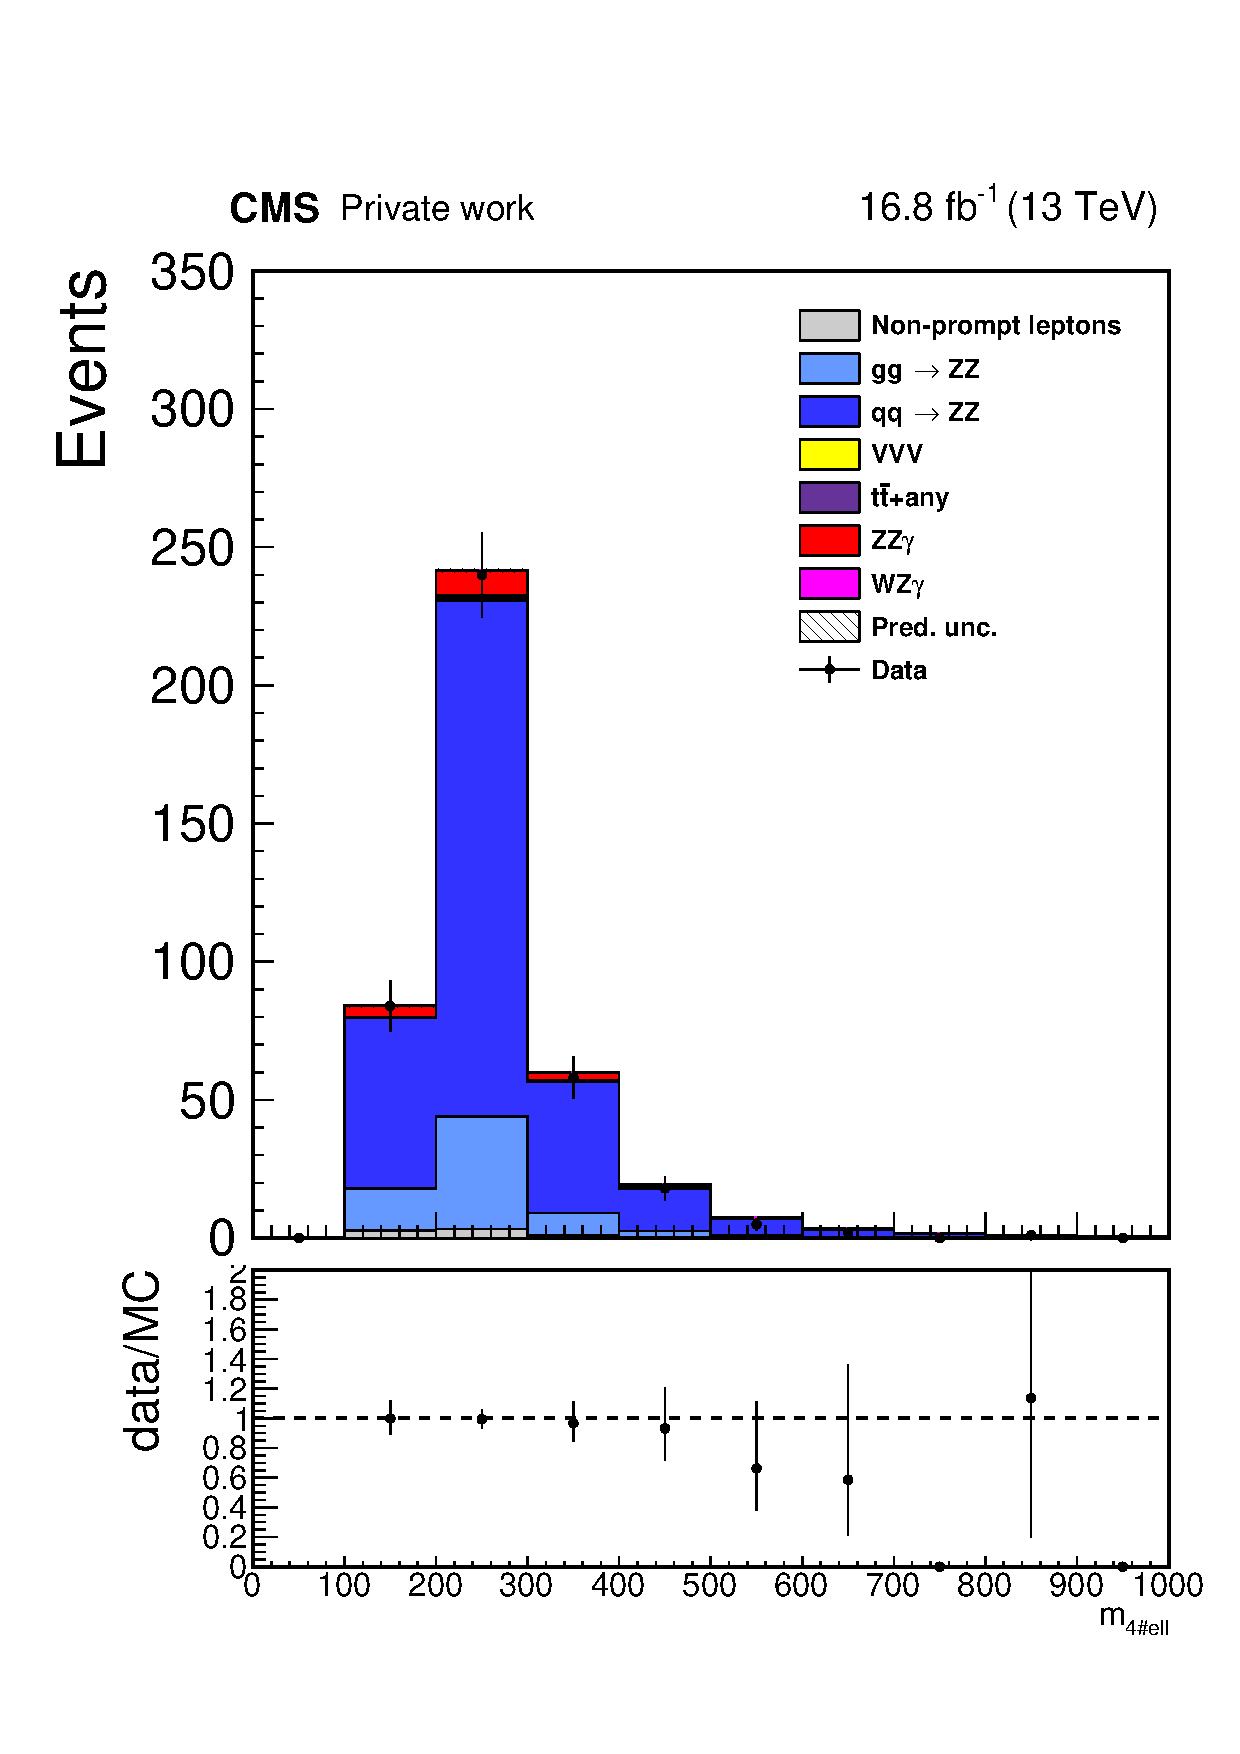
\includegraphics[width=.25\textwidth]{Figures/VVGammaAnalyzer/2016postVFP/lepCR/SR4P/ZZ_mass_pow.pdf}}%
%% \subfigure [2017       ] {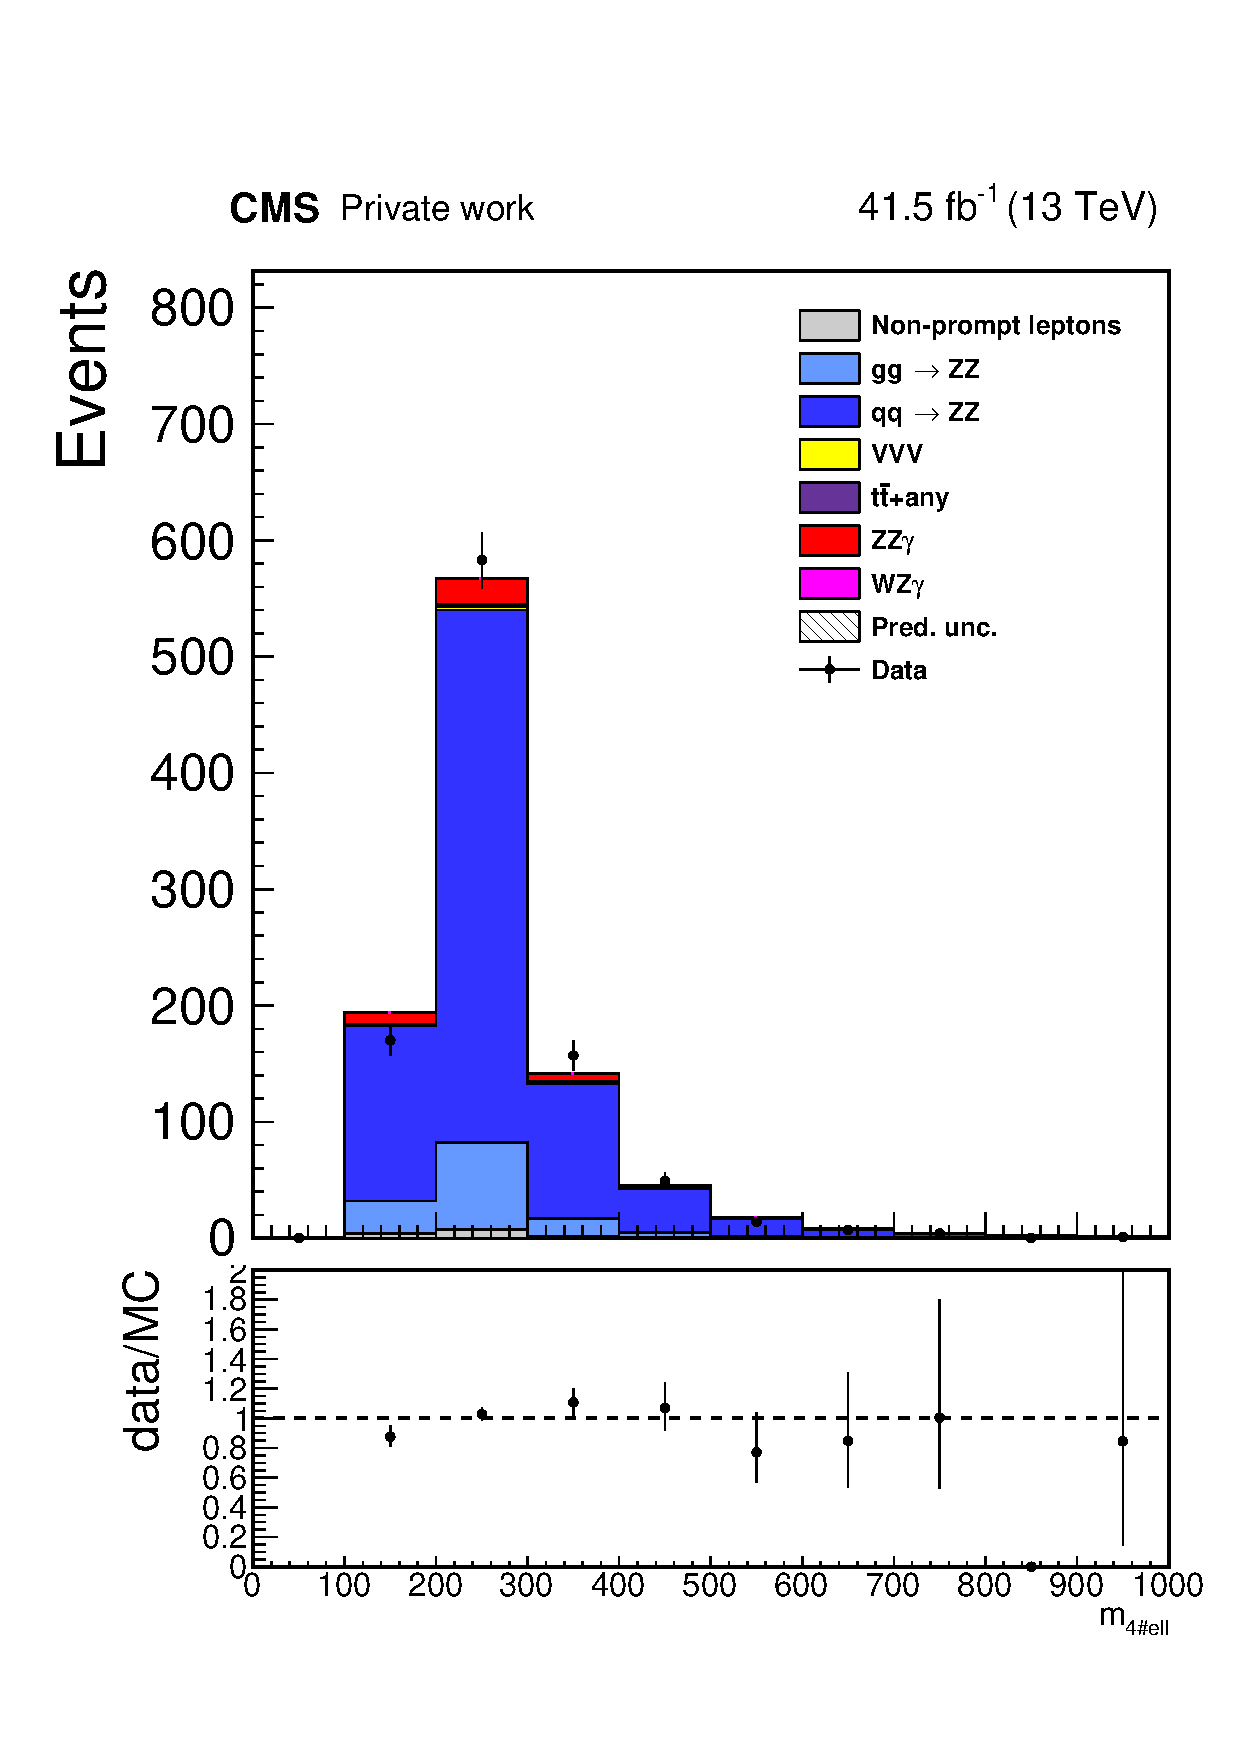
\includegraphics[width=.25\textwidth]{Figures/VVGammaAnalyzer/2017/lepCR/SR4P/ZZ_mass_pow.pdf}}%
%% \subfigure [2018       ] {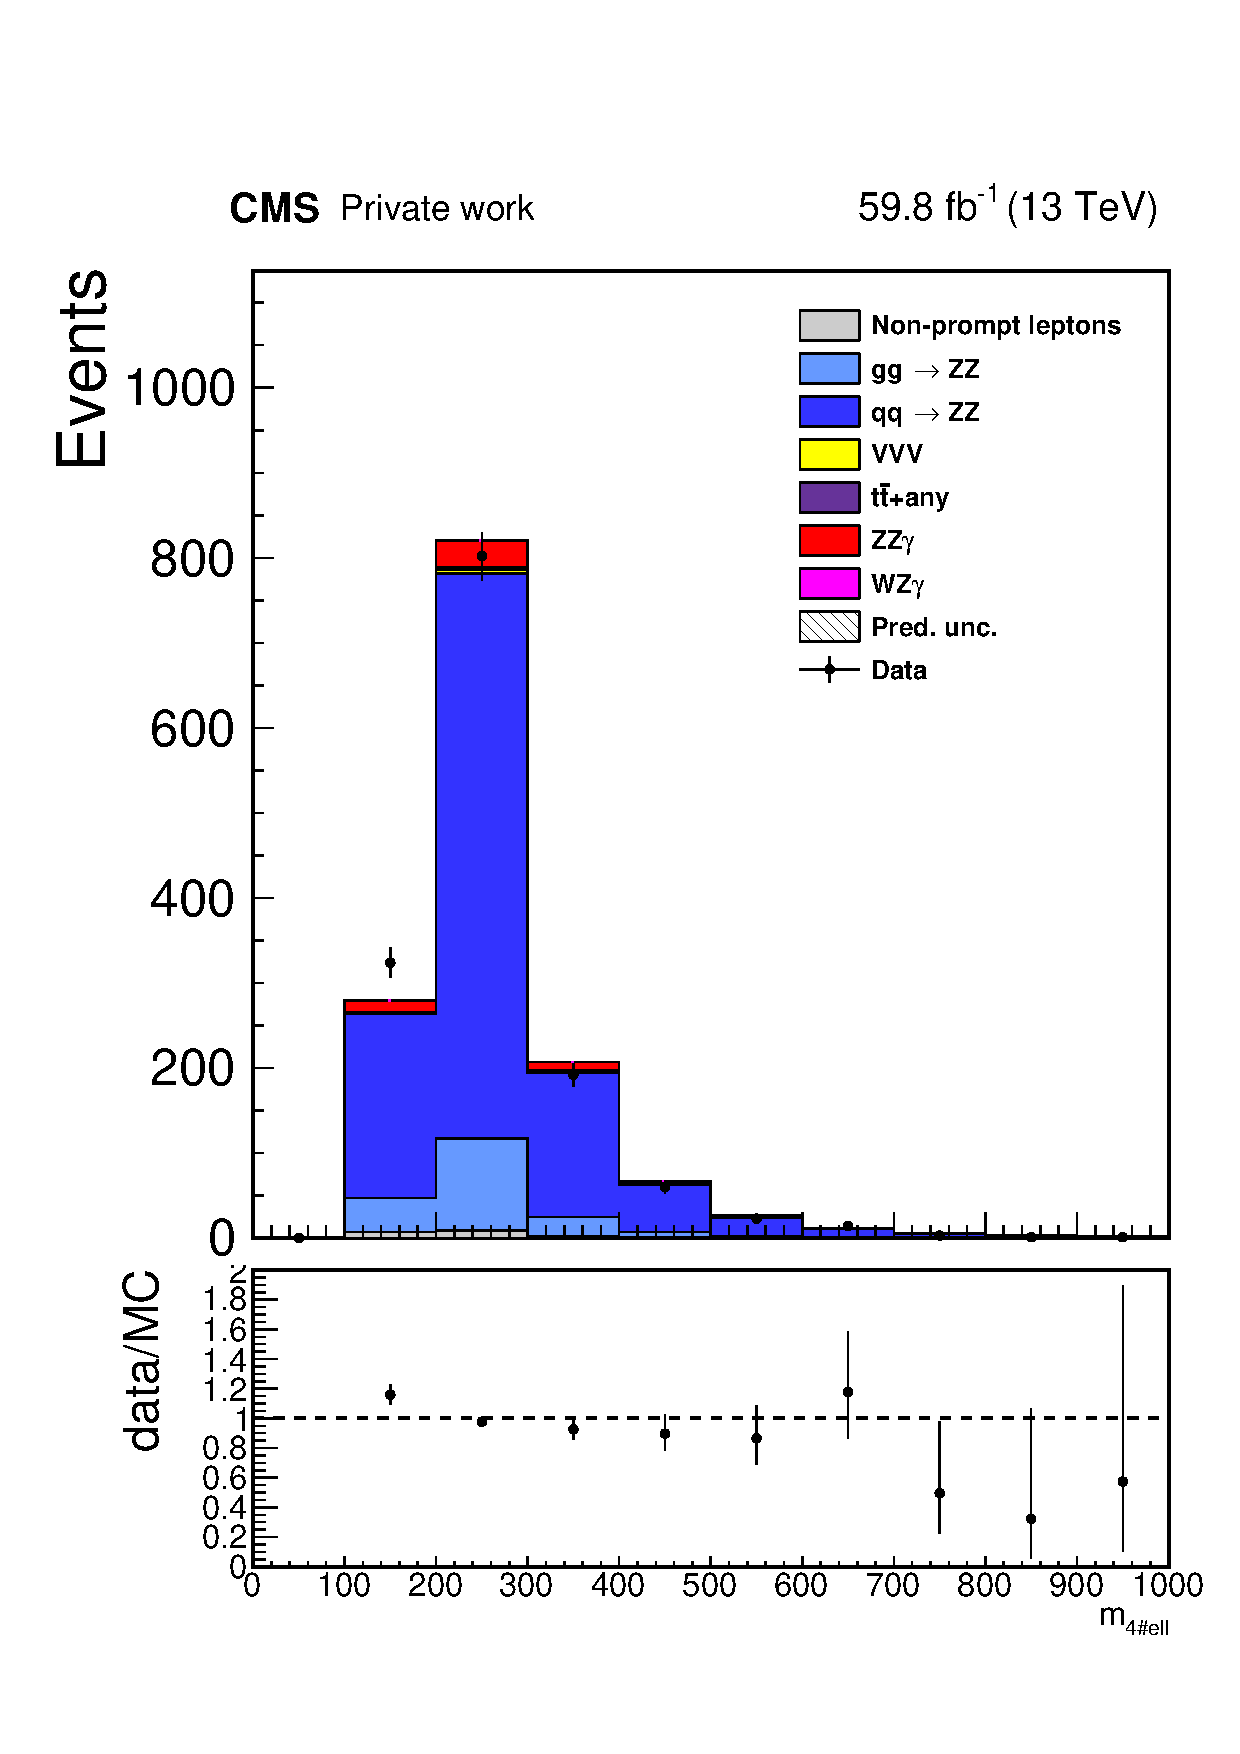
\includegraphics[width=.25\textwidth]{Figures/VVGammaAnalyzer/2018/lepCR/SR4P/ZZ_mass_pow.pdf}}
%% \caption{Invariant mass of the ZZ system, without any requirements on the presence of photons, for each of the data-taking periods of \Run2.}
%% \label{fig:ZZmass_byyear}
%% \end{figure}

%% \begin{figure}
%% \subfigure [$\pt^{\PGg_{\text{FSR}}}$   ] {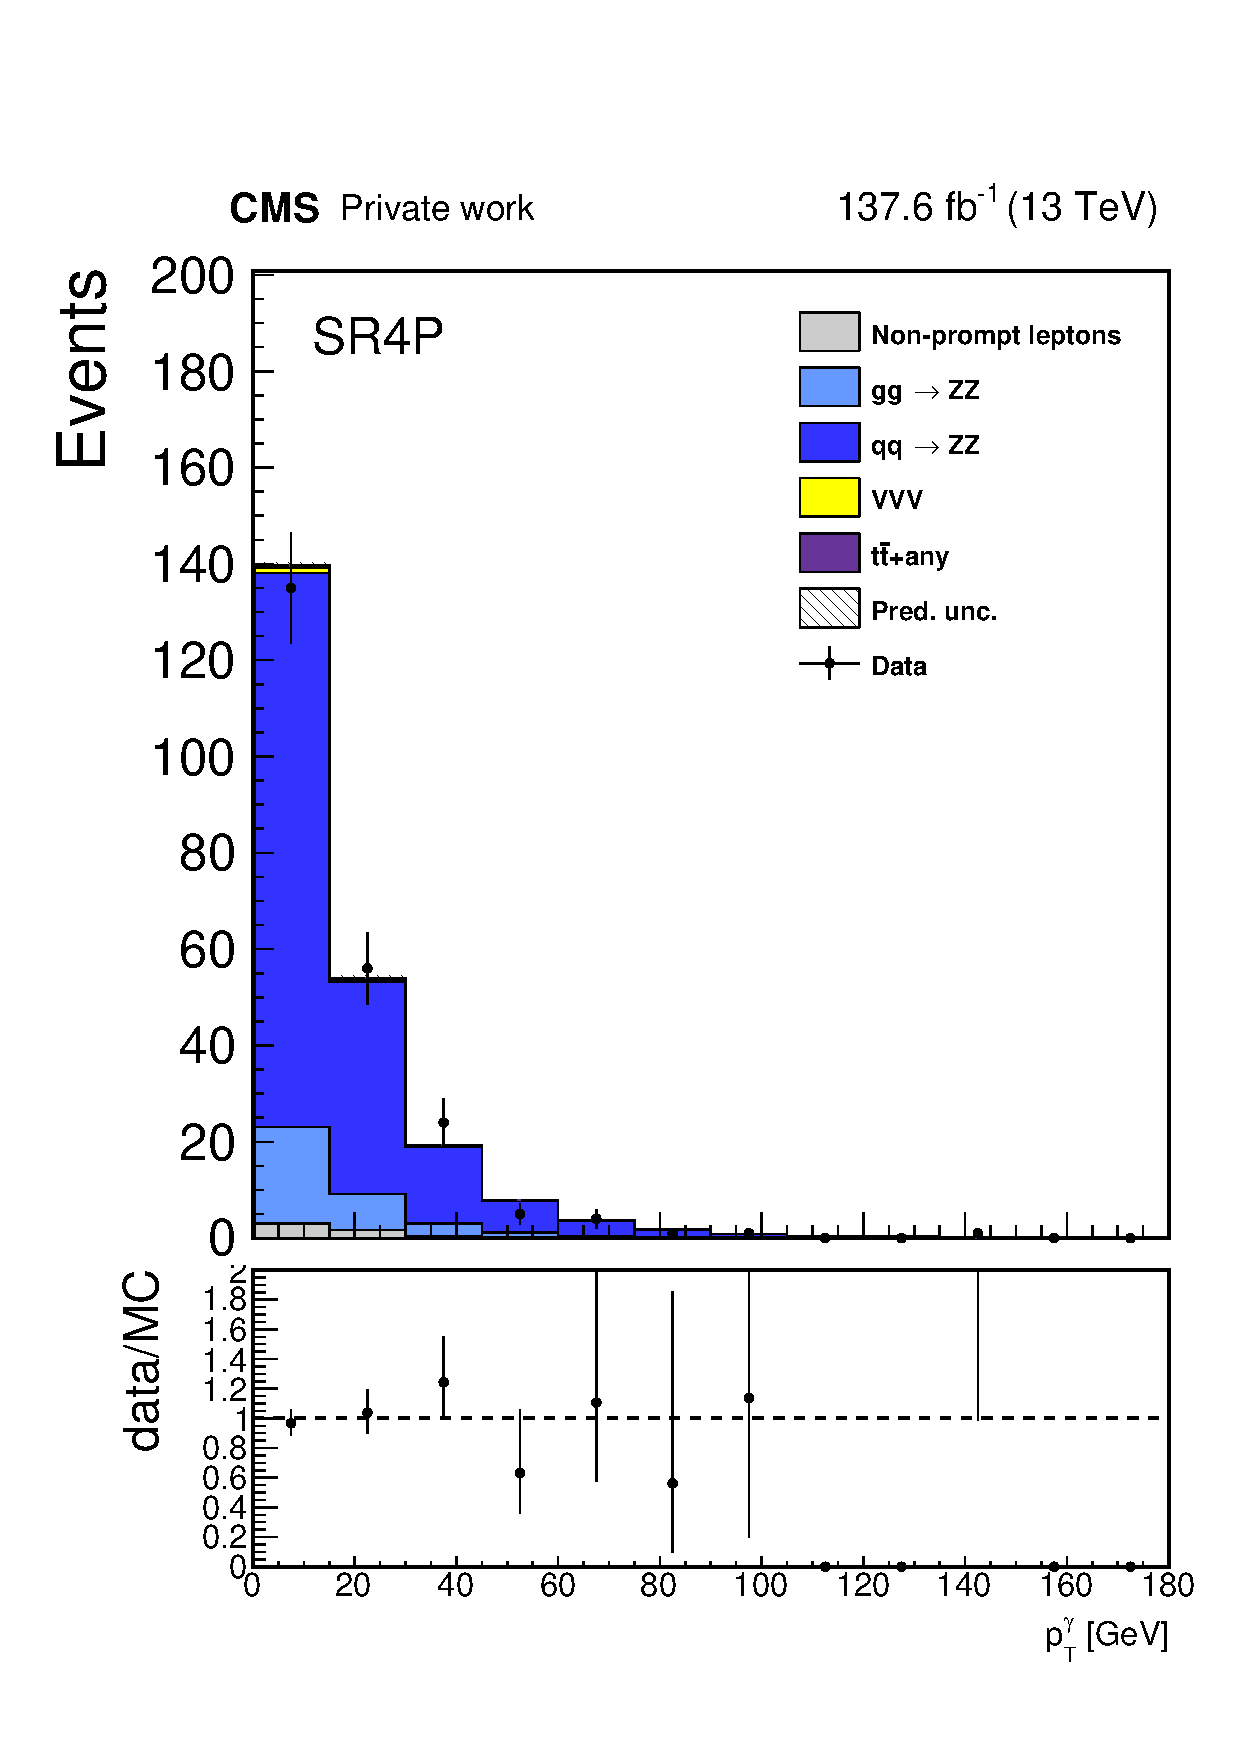
\includegraphics[width=.333333333\textwidth]{Figures/dataMC/Run2/lepCR/SR4P/lead_fsrPhotons_pt_pow.pdf}}%
%% \subfigure [$|\eta^{\PGg_{\text{FSR}}}|$] {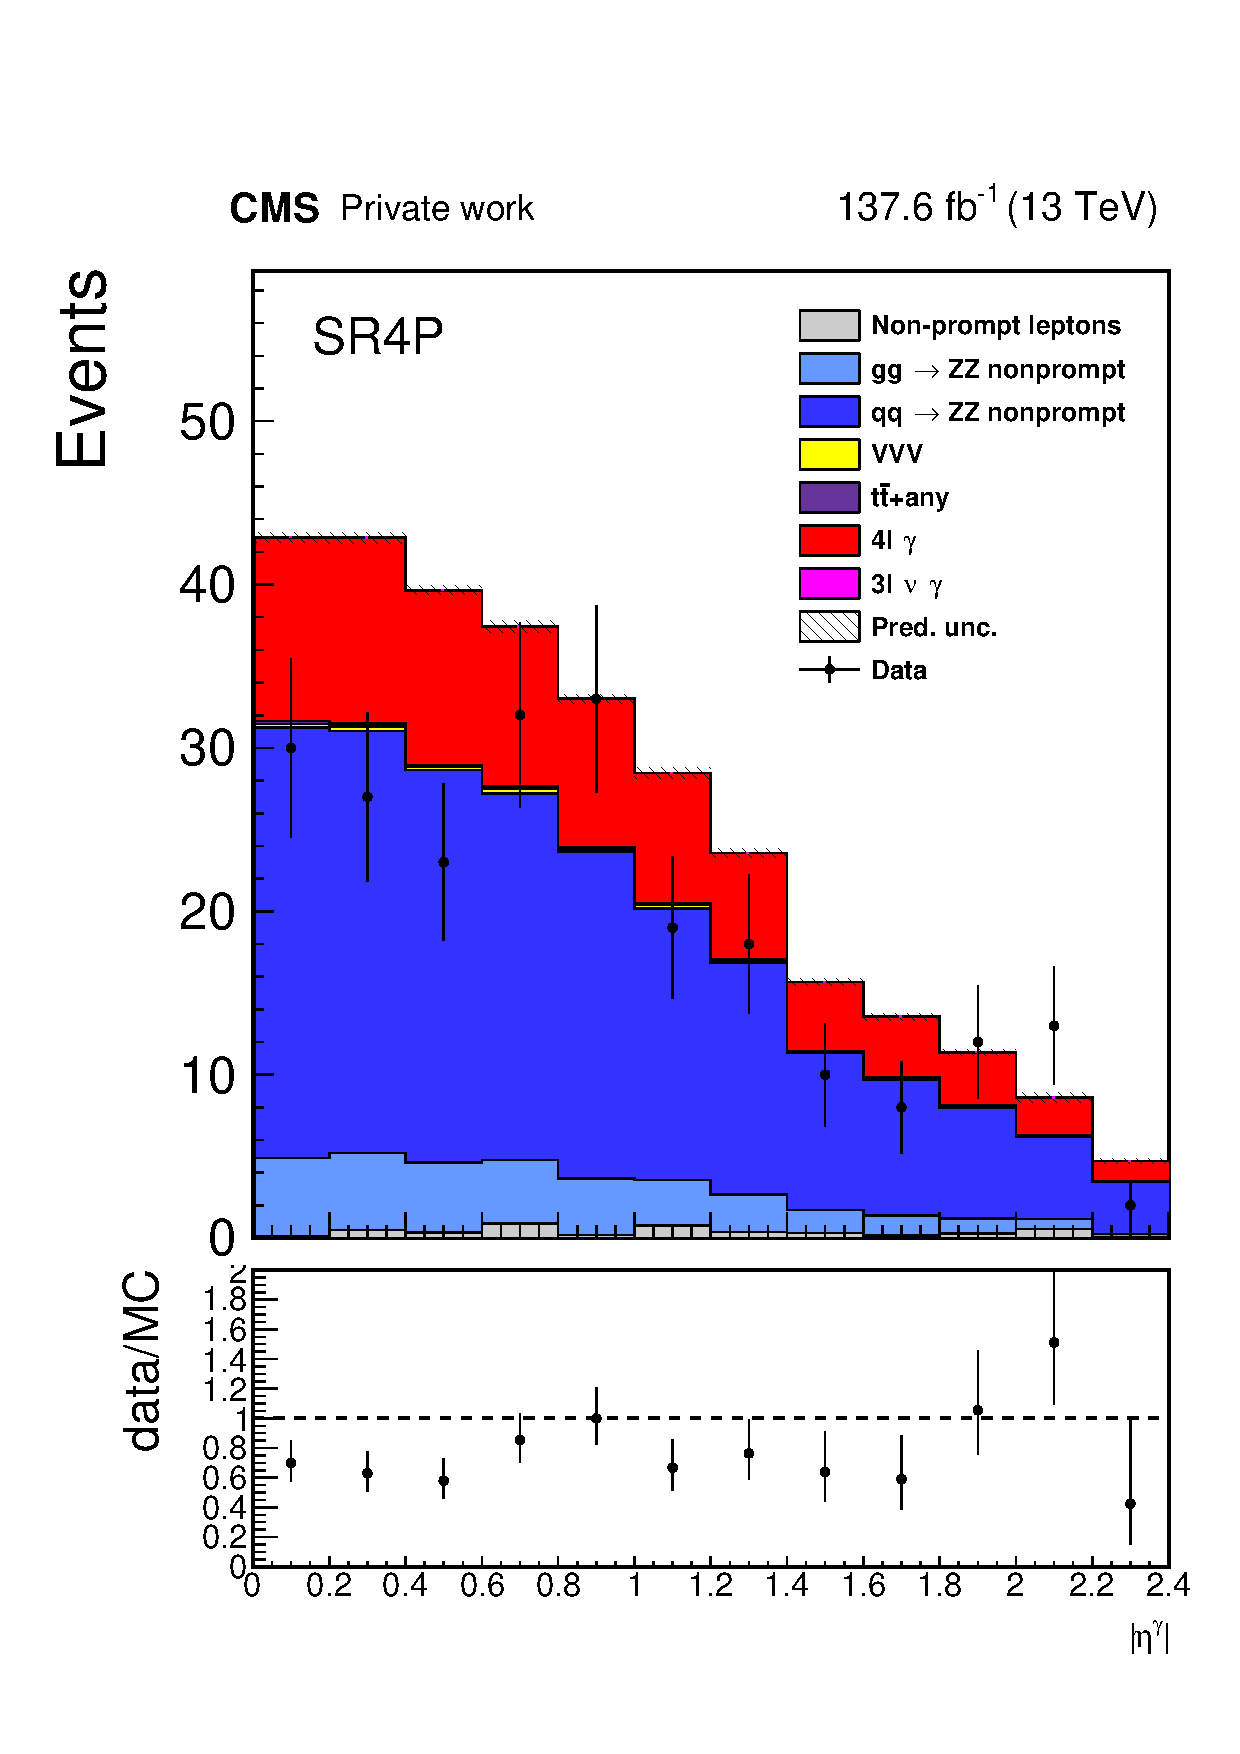
\includegraphics[width=.333333333\textwidth]{Figures/dataMC/Run2/lepCR/SR4P/lead_fsrPhotons_aeta_pow.pdf}}%
%% \subfigure [$\DR(\PGg_{\text{FSR}},\Pl)$] {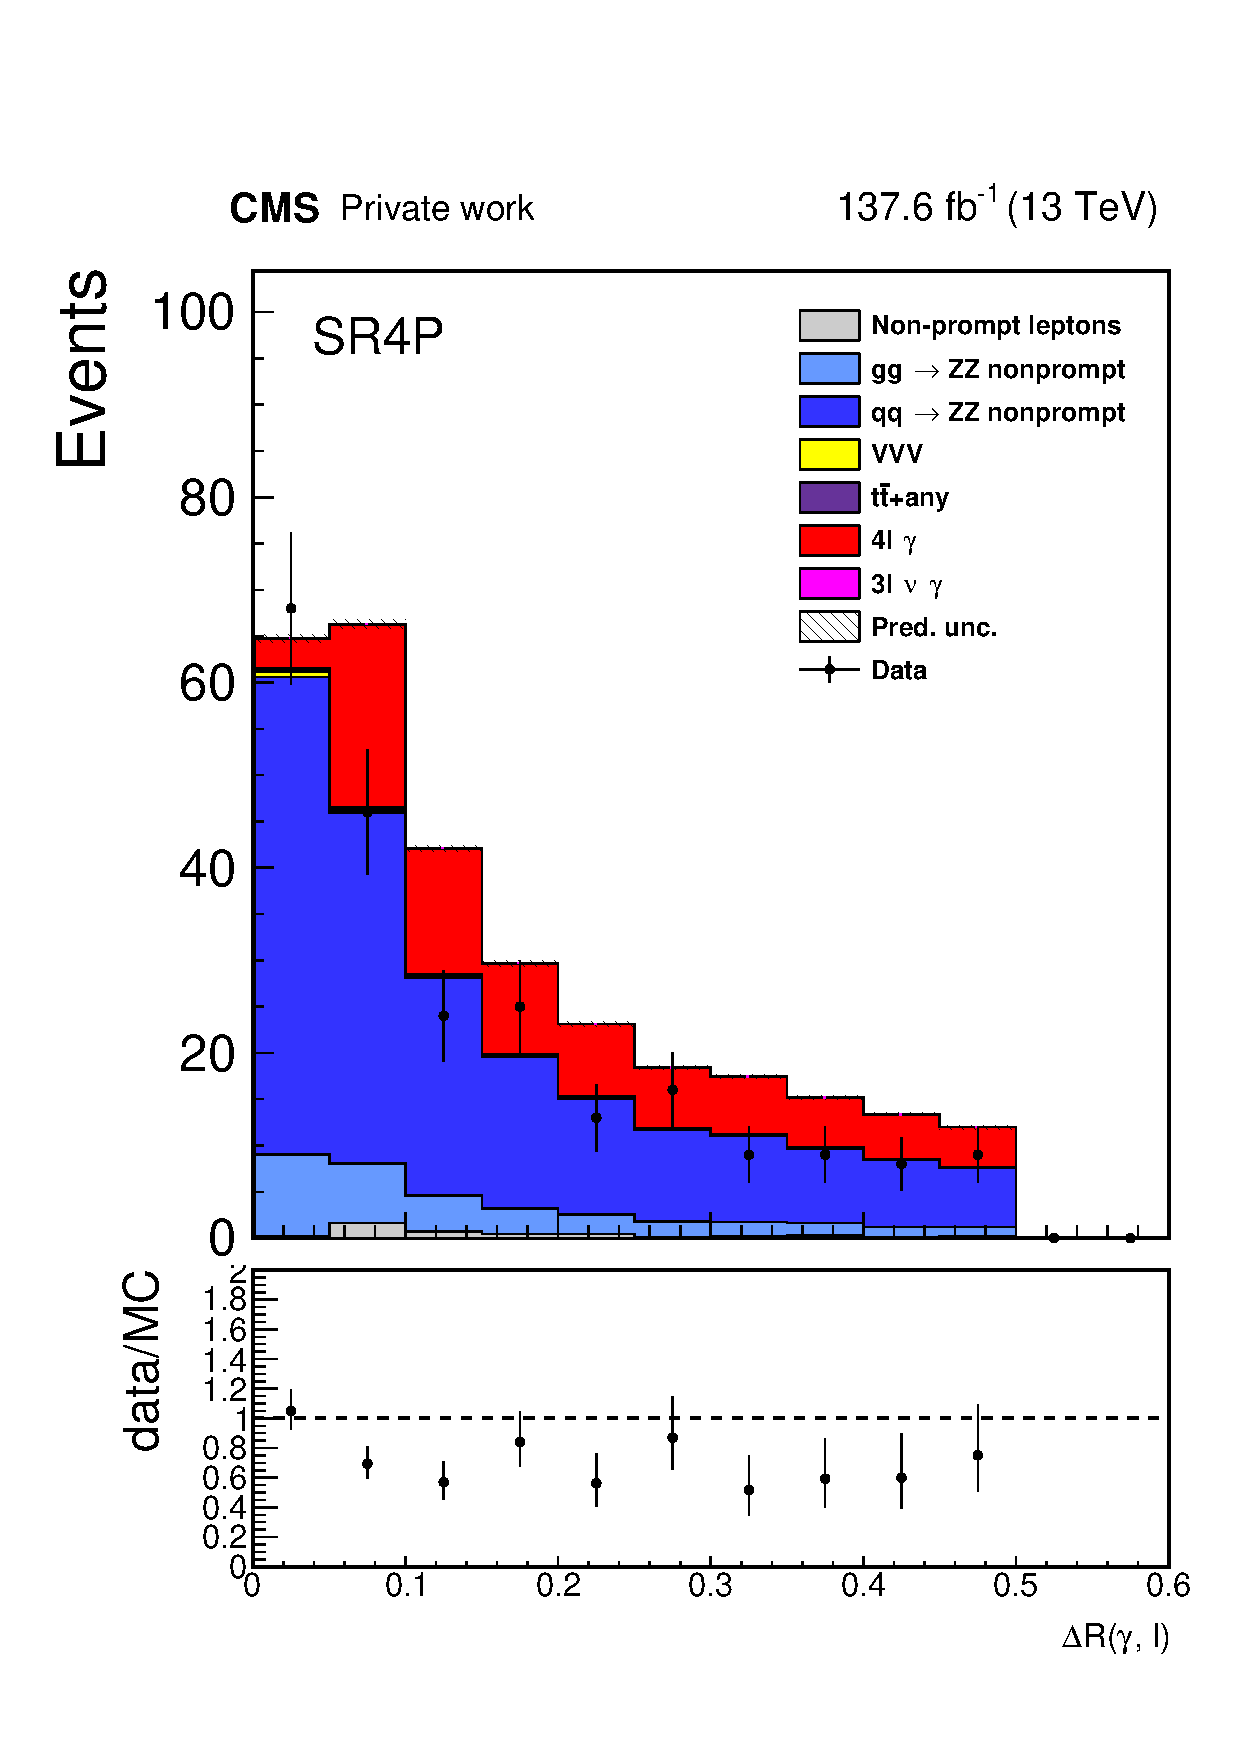
\includegraphics[width=.333333333\textwidth]{Figures/dataMC/Run2/lepCR/SR4P/lead_fsrPhotons_dRl_pow.pdf}}
%% \caption{Transverse momentum (left), pseudorapidity (centre) distance from the associated lepton (right)
%% of most energetic photon that was attached to an electron or muon as part of the FSR recovery algorithm.}
%% \label{fig:Run2_SR4P_fsrPhotons}
%% \end{figure}

\subsection{Three lepton channel}
\label{sec:yields_3L}

The pre-fit yields for the signal and background processes for the signal region of the three lepton channel,
with three leptons passing the tight selection and a photon passing the cut-based ID (SR4P\_1P),
can be seen in Table \ref{tab:Run2_SR3P_phoCR_lepCR} (Table~\ref{tab:Run2_SR3P_phoMC_lepCR})
when using the data-driven (simulation) to estimate tha fake photon background.
The simulation of \nonprompt photons corresponds to the events without a prompt generated photon
in the samples $\PQq\PQq\to\PZ\PZ$, $\Pg\Pg\to\PZ\PZ$, $\PW\PZ\to3\Pl\PGn$ and Drell-Yan.

\begin{table}
  \caption{Yields from the signal region SR3P\_1P, with three leptons passing the tight selection and a photon passing the cut-based ID.
  The \nonprompt and misidentified photons are estimated with the data-driven method
  and thus only the events containing a prompt generated photon are included from the main background samples.
  }
  \label{tab:Run2_SR3P_phoCR_lepCR}
  \resizebox{\textwidth}{!}{%
  \begin{tabular}{l >{$}r<{$} >{$}r<{$} >{$}r<{$} >{$}r<{$} >{$}r<{$}}
    \toprule
    {} & \makecell[c]{\text{2016preVFP}} & \makecell[c]{\text{2016postVFP}} & \makecell[c]{\text{2017}} & \makecell[c]{\text{2018}} & \makecell[c]{\text{\Run2}}\\
    \midrule
    $\PW\PZ\PGg\to3\Pl\PGn\PGg$   &   7.64 \pm 0.07 &   6.89 \pm 0.05 &  17.07 \pm 0.13 &   24.81 \pm 0.19 &   56.42 \pm 0.24 \\
    $\PZ\PZ\PGg\to4\Pl\PGg$       &   1.02 \pm 0.03 &   0.86 \pm 0.03 &   2.55 \pm 0.08 &    3.73 \pm 0.12 &    8.16 \pm 0.15 \\
    Fake photons                  &  18.31 \pm 2.33 &  13.64 \pm 1.86 &  35.05 \pm 2.61 &   55.75 \pm 3.41 &  122.75 \pm 5.23 \\
    $\Pg\Pg\to\PZ\PZ\to4\Pe$      &   0.04 \pm 0.00 &   0.03 \pm 0.00 &   0.10 \pm 0.00 &    0.14 \pm 0.00 &    0.31 \pm 0.00 \\
    $\Pg\Pg\to\PZ\PZ\to2\Pe2\PGm$ &   0.05 \pm 0.00 &   0.04 \pm 0.00 &   0.07 \pm 0.00 &    0.10 \pm 0.00 &    0.25 \pm 0.01 \\
    $\Pg\Pg\to\PZ\PZ\to4\PGm$     &   0.01 \pm 0.00 &   0.01 \pm 0.00 &   0.03 \pm 0.00 &    0.05 \pm 0.00 &    0.11 \pm 0.00 \\
    $\PZ\PGg$                     &   5.33 \pm 0.78 &   4.98 \pm 0.59 &   8.84 \pm 1.40 &   16.52 \pm 2.10 &   35.68 \pm 2.71 \\
    $\PQt\PAQt\PZ$+jets           &   0.06 \pm 0.01 &   0.05 \pm 0.00 &   0.14 \pm 0.01 &    0.18 \pm 0.01 &    0.43 \pm 0.02 \\
    \noalign{\vspace{.3ex}}\hline\noalign{\vspace{.3ex}}
    Total                         &  32.46 \pm 2.46 &  26.50 \pm 1.96 &  63.85 \pm 2.97 &  101.28 \pm 4.01 &  224.10 \pm 5.90 \\
    \bottomrule
  \end{tabular}
  }
\end{table}

\begin{table}
  \caption{Yields from the signal region SR3P\_1P, with three leptons passing the tight selection and a photon passing the cut-based ID.
  The \nonprompt and misidentified photons are estimated from simulation.
  }
  \label{tab:Run2_SR3P_phoMC_lepCR}
  \resizebox{\textwidth}{!}{%
  \begin{tabular}{l >{$}r<{$} >{$}r<{$} >{$}r<{$} >{$}r<{$} >{$}r<{$}}
    \toprule
    {} & \makecell[c]{\text{2016preVFP}} & \makecell[c]{\text{2016postVFP}} & \makecell[c]{\text{2017}} & \makecell[c]{\text{2018}} & \makecell[c]{\text{\Run2}}\\
    \midrule
    \noalign{\vspace{.3ex}}\hline\noalign{\vspace{.3ex}}
    $\PW\PZ\PGg\to3\Pl\PGn\PGg$   &   7.64 \pm 0.07 &   6.89 \pm 0.05 &  17.07 \pm 0.13 &   24.81 \pm 0.19 &   56.42 \pm 0.24 \\
    $\PZ\PZ\PGg\to4\Pl\PGg$       &   1.02 \pm 0.03 &   0.86 \pm 0.03 &   2.55 \pm 0.08 &    3.73 \pm 0.12 &    8.16 \pm 0.15 \\
    \qqZZnonpro                   &   3.89 \pm 0.04 &   2.91 \pm 0.03 &  11.77 \pm 0.08 &   15.87 \pm 0.11 &   34.45 \pm 0.15 \\
    $\Pg\Pg\to\PZ\PZ\to4\Pe$      &   0.23 \pm 0.00 &   0.17 \pm 0.00 &   0.63 \pm 0.01 &    0.95 \pm 0.01 &    1.97 \pm 0.01 \\
    $\Pg\Pg\to\PZ\PZ\to2\Pe2\PGm$ &   0.31 \pm 0.01 &   0.21 \pm 0.00 &   0.42 \pm 0.01 &    0.59 \pm 0.01 &    1.53 \pm 0.01 \\
    $\Pg\Pg\to\PZ\PZ\to4\PGm$     &   0.02 \pm 0.00 &   0.01 \pm 0.00 &   0.04 \pm 0.00 &    0.05 \pm 0.00 &    0.12 \pm 0.00 \\
    \WZnonpro                     &   2.94 \pm 0.30 &   2.28 \pm 0.24 &   7.30 \pm 0.64 &   47.53 \pm 1.86 &   60.05 \pm 2.00 \\
    \ZGprompt                     &   5.33 \pm 0.78 &   4.98 \pm 0.59 &   8.84 \pm 1.40 &   16.52 \pm 2.10 &   35.68 \pm 2.71 \\
    $\PQt\PAQt\PZ$+jets           &   0.11 \pm 0.01 &   0.10 \pm 0.01 &   0.26 \pm 0.01 &    0.34 \pm 0.02 &    0.81 \pm 0.02 \\
    \DYnonpro                     &   0.00 \pm 0.00 &   0.14 \pm 2.61 &   0.00 \pm 0.00 &    3.03 \pm 7.29 &    3.16 \pm 7.74 \\
    Total                         &  21.49 \pm 0.84 &  18.56 \pm 2.69 &  48.87 \pm 1.55 &  113.43 \pm 7.81 &  202.35 \pm 8.45 \\
    \bottomrule
  \end{tabular}
  }
\end{table}

The data-driven prediction of \nonprompt and misidentified photons yields a larger number of events
than the prediction extracted from the simulation.

